\chapter{La Integral Definida}

\section{Antecedentes Históricos: De Arquímedes a Leibniz}

El problema de calcular el área de regiones con fronteras curvas es uno de los más antiguos de la matemática. Los geómetras griegos sabían calcular áreas de polígonos ---dividiendo la figura en triángulos---, pero la extensión de este procedimiento a curvas arbitrarias representaba un obstáculo conceptual de primer orden. La solución más refinada de la antigüedad fue propuesta por \textbf{Arquímedes de Siracusa} (287--212 a.C.) en su tratado \emph{Cuadratura de la parábola} y en \emph{La medida del círculo}: el célebre \textbf{método de exhaución}. La idea consiste en inscribir y circunscribir polígonos regulares de $n$ lados en la región de interés; a medida que $n$ crece, las áreas poligonales acotan al área verdadera por arriba y por abajo con precisión creciente, y el área exacta es el único valor que no puede ser excluido por ninguna aproximación. Arquímedes demostró con este método que el área del círculo de radio $r$ es $\pi r^2$, y que el área bajo la parábola $y = x^2$ entre $0$ y $1$ es $\frac{1}{3}$.

\begin{center}
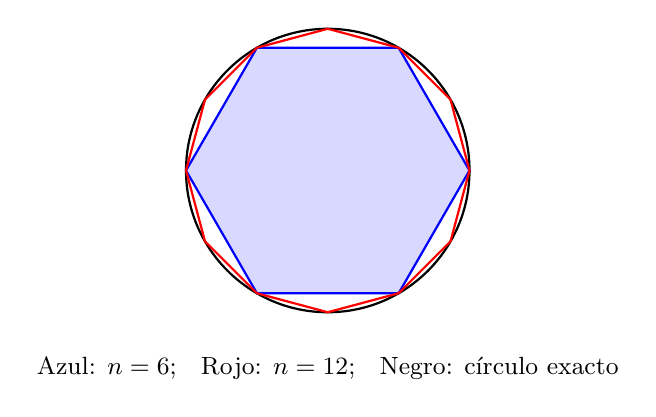
\begin{tikzpicture}[scale=1.8]
    \draw[thick] (0,0) circle (1);
    % Polígono inscrito n=6
    \draw[blue, thick, fill=blue!15]
        (0:1) -- (60:1) -- (120:1) -- (180:1) -- (240:1) -- (300:1) -- cycle;
    % Polígono inscrito n=12
    \draw[red, thick]
        (0:1) -- (30:1) -- (60:1) -- (90:1) -- (120:1) -- (150:1) --
        (180:1) -- (210:1) -- (240:1) -- (270:1) -- (300:1) -- (330:1) -- cycle;
    \node[below] at (0,-1.25)
        {\small Azul: $n=6$; \; Rojo: $n=12$; \; Negro: círculo exacto};
\end{tikzpicture}
\end{center}

\begin{rem}
El método de exhaución de Arquímedes anticipa conceptualmente el límite, aunque sin la formulación algebraica que desarrollarían Newton y Leibniz dos mil años después. Lo que separa a Arquímedes del cálculo moderno no es la intuición, sino el lenguaje simbólico. Fue Gottfried Wilhelm Leibniz quien en 1675 introdujo la notación $\int f(x)\,dx$ ---donde el signo $\int$ es una ``S'' alargada de \emph{summa}--- y estableció las reglas de manipulación de diferenciales que permiten calcular integrales de manera sistemática.
\end{rem}

\section{Notación Sigma y Fórmulas de Sumatorias}

Para formalizar el proceso de aproximación por sumas finitas se utiliza la \textbf{notación sigma}, que permite escribir sumas de muchos términos de forma compacta. La suma $f(x_1) + f(x_2) + \cdots + f(x_n)$ se escribe como $\sum_{i=1}^{n} f(x_i)$.

\begin{theorem}[Fórmulas de sumatorias fundamentales]
Para todo entero positivo $n$:
\[
\sum_{i=1}^{n} 1 = n, \qquad
\sum_{i=1}^{n} i = \frac{n(n+1)}{2}, \qquad
\sum_{i=1}^{n} i^2 = \frac{n(n+1)(2n+1)}{6}, \qquad
\sum_{i=1}^{n} i^3 = \left[\frac{n(n+1)}{2}\right]^2.
\]
\end{theorem}

\begin{rem}
La fórmula $\sum_{i=1}^n i = \frac{n(n+1)}{2}$ se atribuye popularmente a Gauss, quien supuestamente la descubrió de niño al sumar los enteros del 1 al 100. El argumento geométrico es elegante: al escribir la suma en orden creciente y decreciente simultáneamente, cada par suma $n+1$ y hay $n$ pares, dando $\frac{n(n+1)}{2}$.
\end{rem}

\section{Sumas de Riemann}

\begin{definition}
Sea $f$ una función definida en $[a,b]$. Una \textbf{partición} de $[a,b]$ es un conjunto de puntos $P = \{x_0, x_1, \ldots, x_n\}$ con
\[
a = x_0 < x_1 < x_2 < \cdots < x_n = b.
\]
La longitud del $i$-ésimo subintervalo es $\Delta x_i = x_i - x_{i-1}$. La \textbf{norma} de la partición es $\|P\| = \max_{1\leq i \leq n} \Delta x_i$. En cada subintervalo $[x_{i-1}, x_i]$ se elige un \textbf{punto muestra} $\bar{x}_i \in [x_{i-1}, x_i]$. La \textbf{suma de Riemann} asociada es
\[
R_P = \sum_{i=1}^{n} f(\bar{x}_i)\,\Delta x_i.
\]
\end{definition}

Geométricamente, cada término $f(\bar{x}_i)\,\Delta x_i$ es el área con signo de un rectángulo de base $\Delta x_i$ y altura $f(\bar{x}_i)$: positiva si $f(\bar{x}_i) > 0$, negativa si $f(\bar{x}_i) < 0$.

\begin{center}
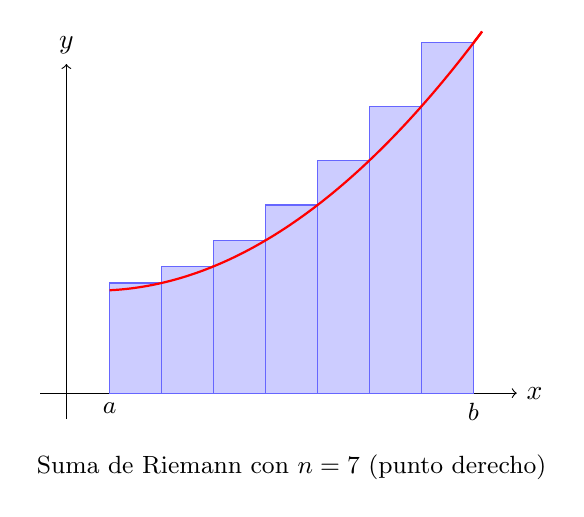
\begin{tikzpicture}[scale=1.1]
    \draw[->] (-0.3,0) -- (5.2,0) node[right] {$x$};
    \draw[->] (0,-0.3) -- (0,3.8) node[above] {$y$};
    % Curva
    \draw[red, thick, domain=0.5:4.8, samples=100]
        plot (\x, {0.15*\x*\x - 0.1*\x + 1.2});
    % Rectángulos (punto derecho)
    \foreach \i in {1,2,3,4,5,6,7} {
        \pgfmathsetmacro\xa{0.5 + (\i-1)*0.6}
        \pgfmathsetmacro\xb{0.5 + \i*0.6}
        \pgfmathsetmacro\ht{0.15*\xb*\xb - 0.1*\xb + 1.2}
        \draw[fill=blue!20, draw=blue!60]
            (\xa,0) rectangle (\xb,\ht);
    }
    % Redibujar curva encima
    \draw[red, thick, domain=0.5:4.8, samples=100]
        plot (\x, {0.15*\x*\x - 0.1*\x + 1.2});
    % Etiquetas
    \node[below] at (0.5,0) {\small $a$};
    \node[below] at (4.7,0) {\small $b$};
    \node[below] at (2.6,-0.6)
        {\small Suma de Riemann con $n = 7$ (punto derecho)};
\end{tikzpicture}
\end{center}

\begin{rem}
Según la elección del punto muestra $\bar{x}_i$, la suma de Riemann toma nombres especiales. Si $\bar{x}_i = x_{i-1}$ se llama \textbf{suma por la izquierda}; si $\bar{x}_i = x_i$, \textbf{suma por la derecha}; si $\bar{x}_i = \frac{x_{i-1}+x_i}{2}$, \textbf{suma del punto medio}. Para funciones monótonas, las sumas por la izquierda y por la derecha proporcionan cotas inferior y superior del área exacta, lo que da lugar a las \textbf{sumas de Darboux}.
\end{rem}

\begin{example}[Integral definida como límite de sumas de Riemann]
Evaluar $\displaystyle\int_{-2}^{3} (x+3)\,dx$ como límite de sumas de Riemann usando puntos derechos.

\begin{myproof}

\textbf{Paso 1: Establecer la partición y los puntos muestrales.}

Tomamos una partición regular con $n$ subintervalos: $\Delta x = \frac{3-(-2)}{n} = \frac{5}{n}$ y puntos derechos $x_i = -2 + i\,\Delta x = -2 + \frac{5i}{n}$. La suma de Riemann es
\[
R_n = \sum_{i=1}^{n} f(x_i)\,\Delta x
= \sum_{i=1}^{n} \left[\left(-2+\frac{5i}{n}\right)+3\right]\frac{5}{n}
= \frac{5}{n}\sum_{i=1}^{n}\left(1 + \frac{5i}{n}\right).
\]

\textbf{Paso 2: Simplificar usando fórmulas de sumatoria.}
\[
R_n = \frac{5}{n}\left[\sum_{i=1}^{n}1 + \frac{5}{n}\sum_{i=1}^{n}i\right]
= \frac{5}{n}\left[n + \frac{5}{n}\cdot\frac{n(n+1)}{2}\right]
= 5 + \frac{25(n+1)}{2n}
= 5 + \frac{25}{2}\left(1+\frac{1}{n}\right).
\]

\textbf{Paso 3: Tomar el límite.}
\[
\boxed{\int_{-2}^{3}(x+3)\,dx = \lim_{n\to\infty} R_n = 5 + \frac{25}{2} = \frac{35}{2}.}
\]
Este resultado puede verificarse geométricamente: la región es un trapecio de bases $f(-2)=1$ y $f(3)=6$ y altura $5$, cuya área es $\frac{(1+6)\cdot 5}{2} = \frac{35}{2}$.
\end{myproof}
\end{example}

\section{La Integral Definida}

\begin{definition}
Sea $f$ definida en $[a,b]$. Se dice que $f$ es \textbf{integrable en $[a,b]$} si el límite
\[
\int_{a}^{b} f(x)\,dx \;=\; \lim_{\|P\|\to 0} \sum_{i=1}^{n} f(\bar{x}_i)\,\Delta x_i
\]
existe y es el mismo para toda elección de particiones con $\|P\|\to 0$ y para toda elección de puntos muestra $\bar{x}_i$. Este límite se denomina la \textbf{integral definida} de $f$ en $[a,b]$.
\end{definition}

\begin{theorem}[Integrabilidad de funciones continuas]
Si $f$ es continua en $[a,b]$, entonces $f$ es integrable en $[a,b]$. Más aún, $f$ es integrable en $[a,b]$ si es acotada y tiene a lo sumo un número finito de discontinuidades.
\end{theorem}

\begin{rem}
La interpretación geométrica de la integral definida depende del signo de $f$. Si $f(x)\geq 0$ en $[a,b]$, la integral representa el área de la región comprendida entre la gráfica de $f$ y el eje $x$. Si $f$ toma valores negativos en alguna parte del intervalo, la integral representa el \textbf{área neta}: el área de las regiones sobre el eje $x$ menos el área de las regiones bajo el eje $x$.
\end{rem}

\begin{center}
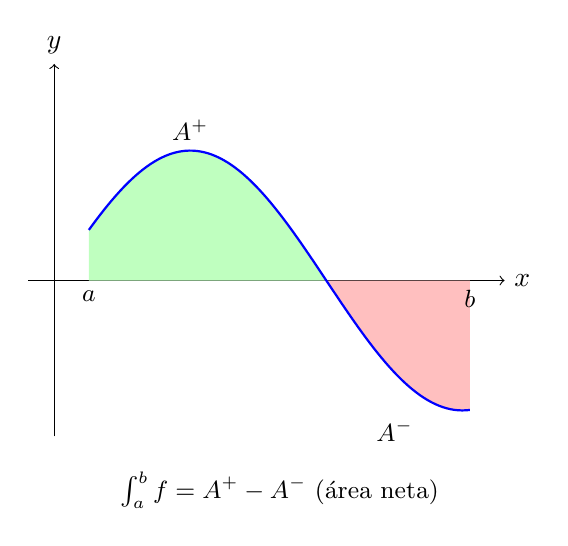
\begin{tikzpicture}[scale=1.1]
    \draw[->] (-0.3,0) -- (5.2,0) node[right] {$x$};
    \draw[->] (0,-1.8) -- (0,2.5) node[above] {$y$};
    % Región positiva (verde)
    \fill[green!25, domain=0.4:3.14, samples=100]
        plot (\x, {1.5*sin(\x r)}) -- (3.14,0) -- (0.4,0) -- cycle;
    % Región negativa (rojo)
    \fill[red!25, domain=3.14:4.8, samples=100]
        plot (\x, {1.5*sin(\x r)}) -- (4.8,0) -- (3.14,0) -- cycle;
    % Curva
    \draw[blue, thick, domain=0.4:4.8, samples=100]
        plot (\x, {1.5*sin(\x r)});
    % Etiquetas
    \node[below] at (0.4,0) {\small $a$};
    \node[below] at (4.8,0) {\small $b$};
    \node[above] at (1.57, 1.5) {\small $A^+$};
    \node[below] at (3.93,-1.5) {\small $A^-$};
    \node[below] at (2.6,-2.1)
        {\small $\int_a^b f = A^+ - A^-$ (área neta)};
\end{tikzpicture}
\end{center}

\section{Propiedades de la Integral Definida}

\begin{theorem}[Propiedades algebraicas]
Sean $f$ y $g$ integrables en $[a,b]$ y $k \in \R$. Entonces:
\begin{enumerate}
    \item $\displaystyle\int_{a}^{b} k\,f(x)\,dx = k\int_{a}^{b} f(x)\,dx$.
    \item $\displaystyle\int_{a}^{b} [f(x) \pm g(x)]\,dx = \int_{a}^{b} f(x)\,dx \pm \int_{a}^{b} g(x)\,dx$.
    \item $\displaystyle\int_{a}^{a} f(x)\,dx = 0$.
    \item $\displaystyle\int_{a}^{b} f(x)\,dx = -\int_{b}^{a} f(x)\,dx$.
\end{enumerate}
\end{theorem}

\begin{theorem}[Aditividad en intervalos]
Si $f$ es integrable en un intervalo que contiene a $a$, $b$ y $c$ (en cualquier orden), entonces
\[
\int_{a}^{b} f(x)\,dx = \int_{a}^{c} f(x)\,dx + \int_{c}^{b} f(x)\,dx.
\]
\end{theorem}

\begin{theorem}[Simetría para funciones pares e impares]
Sea $f$ integrable en $[-a, a]$ con $a > 0$.
\begin{enumerate}
    \item Si $f$ es \textbf{par} ($f(-x) = f(x)$): $\displaystyle\int_{-a}^{a} f(x)\,dx = 2\int_{0}^{a} f(x)\,dx$.
    \item Si $f$ es \textbf{impar} ($f(-x) = -f(x)$): $\displaystyle\int_{-a}^{a} f(x)\,dx = 0$.
\end{enumerate}
\end{theorem}

\begin{rem}
Las propiedades de simetría reducen significativamente el trabajo algebraico en integrales sobre intervalos simétricos. Por ejemplo, $\int_{-\pi}^{\pi}\sen^3 x\,dx = 0$ sin necesidad de calcular nada, pues $\sen^3 x$ es función impar.
\end{rem}

\begin{theorem}[Propiedad de acotamiento y comparación]
Sea $f$ integrable en $[a,b]$ con $a < b$.
\begin{enumerate}
    \item Si $m \leq f(x) \leq M$ para todo $x\in[a,b]$, entonces
    \[
    m(b-a) \leq \int_{a}^{b} f(x)\,dx \leq M(b-a).
    \]
    \item Si $f(x) \leq g(x)$ para todo $x\in[a,b]$, entonces $\displaystyle\int_{a}^{b} f(x)\,dx \leq \int_{a}^{b} g(x)\,dx$.
    \item $\displaystyle\left|\int_{a}^{b} f(x)\,dx\right| \leq \int_{a}^{b} |f(x)|\,dx$.
\end{enumerate}
\end{theorem}

\begin{example}[Acotamiento de una integral definida]
Acotar $\displaystyle\int_{2}^{4} x^2\,dx$ sin calcularla directamente.

\begin{myproof}

\textbf{Paso 1: Identificar el mínimo y máximo de $f$ en $[2,4]$.}

En $[2,4]$, la función $f(x) = x^2$ es creciente, por lo que $m = f(2) = 4$ y $M = f(4) = 16$.

\textbf{Paso 2: Aplicar la propiedad de acotamiento.}
\[
4(4-2) \leq \int_{2}^{4} x^2\,dx \leq 16(4-2), \qquad \text{es decir}:
\]
\[
\boxed{8 \leq \int_{2}^{4} x^2\,dx \leq 32.}
\]
El valor exacto es $\left[\frac{x^3}{3}\right]_2^4 = \frac{64}{3} - \frac{8}{3} = \frac{56}{3} \approx 18.67$, que efectivamente cae en el intervalo $[8,32]$.
\end{myproof}
\end{example}

\section{Los Teoremas Fundamentales del Cálculo}

El resultado más importante del análisis elemental es la conexión entre las dos operaciones que parecían independientes: la diferenciación y la integración. Esta relación, descubierta independientemente por Newton y Leibniz en el siglo XVII, constituye el núcleo de todo el cálculo.

\subsection{Primer Teorema Fundamental}

\begin{definition}
Sea $f$ continua en $[a,b]$. La \textbf{función de acumulación} (o función de área) asociada a $f$ es
\[
F(x) = \int_{a}^{x} f(t)\,dt, \qquad x \in [a,b].
\]
\end{definition}

\begin{center}
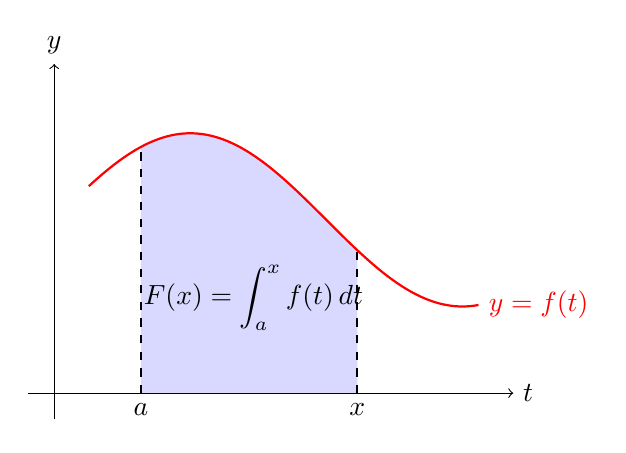
\begin{tikzpicture}[scale=1.1]
    \fill[blue!15, domain=1:3.5, samples=100]
        plot (\x, {sin(\x r) + 2}) -- (3.5,0) -- (1,0) -- cycle;
    \draw[->] (-0.3,0) -- (5.3,0) node[right] {$t$};
    \draw[->] (0,-0.3) -- (0,3.8) node[above] {$y$};
    \draw[red, thick, domain=0.4:4.9, samples=100]
        plot (\x, {sin(\x r) + 2}) node[right] {$y=f(t)$};
    \draw[dashed, thick] (1,0) node[below] {$a$} -- (1,{sin(1 r)+2});
    \draw[dashed, thick] (3.5,0) node[below] {$x$} -- (3.5,{sin(3.5 r)+2});
    \node at (2.3,1.1) {$F(x)=\displaystyle\int_a^x f(t)\,dt$};
\end{tikzpicture}
\end{center}

\begin{theorem}[Primer Teorema Fundamental del Cálculo --- TFC1]
Si $f$ es continua en $[a,b]$, entonces la función de acumulación $F(x) = \int_{a}^{x} f(t)\,dt$ es diferenciable en $(a,b)$ y
\[
F'(x) = \frac{d}{dx}\left[\int_{a}^{x} f(t)\,dt\right] = f(x).
\]
\end{theorem}

El TFC1 afirma que la tasa de cambio instantánea del área acumulada bajo $f$ hasta el punto $x$ es exactamente el valor de $f$ en ese punto: si la función es grande en $x$, el área crece rápidamente; si es pequeña, crece despacio.

\begin{example}[Derivada de una función de acumulación (TFC1)]
Si $F(x) = \int_{1}^{x} t^3\,dt$, calcular $F'(x)$.

\begin{myproof}

\textbf{Paso 1: Aplicar el TFC1.}

Por el TFC1, simplemente se sustituye $t = x$ en el integrando:
\[
\boxed{F'(x) = x^3.}
\]
\end{myproof}
\end{example}

\begin{example}[TFC1 con regla de la cadena]
Calcular $\dfrac{d}{dx}\displaystyle\int_{2}^{x^2} \frac{t^{3/2}}{\sqrt{t^2+17}}\,dt$.

\begin{myproof}

\textbf{Paso 1: Identificar el límite superior variable y definir la función auxiliar.}

El límite superior es $u(x) = x^2$, una función de $x$. Definimos $G(u) = \int_2^u \frac{t^{3/2}}{\sqrt{t^2+17}}\,dt$, de modo que la expresión pedida es $G(u(x))$.

\textbf{Paso 2: Aplicar TFC1 y la regla de la cadena.}
\[
\boxed{\frac{d}{dx}\int_{2}^{x^2} \frac{t^{3/2}}{\sqrt{t^2+17}}\,dt = \frac{(x^2)^{3/2}}{\sqrt{(x^2)^2+17}}\cdot 2x = \frac{2x^4}{\sqrt{x^4+17}}.}
\]
\end{myproof}
\end{example}

\begin{rem}
La forma general de aplicación del TFC1 con regla de la cadena es:
\[
\frac{d}{dx}\int_{g(x)}^{h(x)} f(t)\,dt = f(h(x))\cdot h'(x) - f(g(x))\cdot g'(x).
\]
\end{rem}

\subsection{Segundo Teorema Fundamental}

\begin{theorem}[Segundo Teorema Fundamental del Cálculo --- TFC2]
Si $f$ es continua en $[a,b]$ y $G$ es \textbf{cualquier antiderivada} de $f$ en $[a,b]$ (es decir, $G' = f$), entonces
\[
\int_{a}^{b} f(x)\,dx = G(b) - G(a) \;=\; \Big[G(x)\Big]_{a}^{b}.
\]
\end{theorem}

Este teorema transforma el cálculo de áreas en un problema algebraico: basta hallar una antiderivada de $f$ y evaluar la diferencia en los extremos. La notación $\Big[G(x)\Big]_a^b$ es estándar y representa $G(b) - G(a)$.

\begin{example}[Integral definida por el TFC2]
Calcular $\displaystyle\int_{0}^{2}(2x^2 - 3x + 2)\,dx$.

\begin{myproof}

\textbf{Paso 1: Hallar una antiderivada.}

Una antiderivada de $2x^2 - 3x + 2$ es $G(x) = \frac{2x^3}{3} - \frac{3x^2}{2} + 2x$.

\textbf{Paso 2: Evaluar en los límites de integración (TFC2).}
\[
\int_{0}^{2}(2x^2-3x+2)\,dx = \left[\frac{2x^3}{3} - \frac{3x^2}{2} + 2x\right]_0^2
= \left(\frac{16}{3} - 6 + 4\right) - 0 = \frac{16}{3} - 2.
\]

\textbf{Paso 3: Simplificar.}
\[
\boxed{\int_{0}^{2}(2x^2 - 3x + 2)\,dx = \frac{10}{3}.}
\]
\end{myproof}
\end{example}

\begin{example}[Integral definida por sustitución]
Calcular $\displaystyle\int_{0}^{1}\frac{x+1}{(x^2+2x+6)^2}\,dx$ usando sustitución.

\begin{myproof}

\textbf{Paso 1: Elegir la sustitución y calcular $du$.}

Sea $u = x^2 + 2x + 6$, de modo que $du = (2x+2)\,dx = 2(x+1)\,dx$, es decir, $(x+1)\,dx = \frac{du}{2}$.

\textbf{Paso 2: Cambiar los límites de integración.}

Para $x=0$: $u=6$; para $x=1$: $u = 1+2+6 = 9$.

\textbf{Paso 3: Evaluar la integral transformada.}
\[
\int_{0}^{1}\frac{x+1}{(x^2+2x+6)^2}\,dx
= \frac{1}{2}\int_{6}^{9} u^{-2}\,du
= \frac{1}{2}\left[-\frac{1}{u}\right]_6^9
= \frac{1}{2}\left(-\frac{1}{9}+\frac{1}{6}\right)
= \frac{1}{2}\cdot\frac{1}{18}.
\]
\[
\boxed{\int_{0}^{1}\frac{x+1}{(x^2+2x+6)^2}\,dx = \frac{1}{36}.}
\]
\end{myproof}
\end{example}

\section{Teorema del Valor Medio para Integrales}

\begin{definition}
Si $f$ es integrable en $[a,b]$, el \textbf{valor promedio} de $f$ en $[a,b]$ es
\[
\bar{f} = \frac{1}{b-a}\int_{a}^{b} f(x)\,dx.
\]
\end{definition}

\begin{theorem}[Teorema del Valor Medio para Integrales]
Si $f$ es continua en $[a,b]$, entonces existe al menos un número $c \in (a,b)$ tal que
\[
f(c) = \frac{1}{b-a}\int_{a}^{b} f(x)\,dx, \qquad \text{equivalentemente,} \qquad \int_{a}^{b} f(x)\,dx = f(c)(b-a).
\]
\end{theorem}

\begin{center}
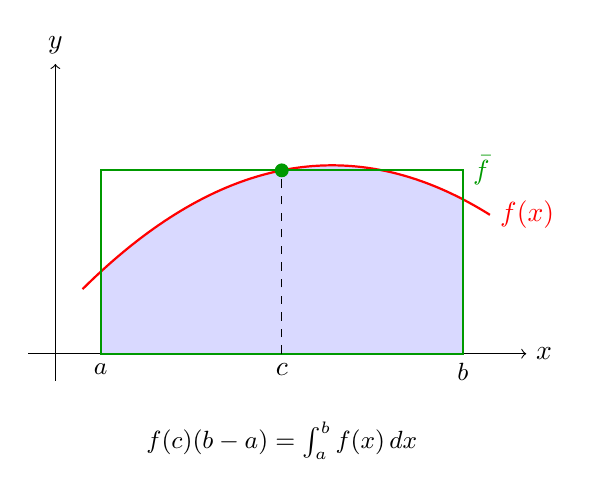
\begin{tikzpicture}[scale=1.15]
    % Área bajo la curva
    \fill[blue!15, domain=0.5:4.5, samples=100]
        plot (\x, {-0.18*\x*\x + 1.1*\x + 0.4}) -- (4.5,0) -- (0.5,0) -- cycle;
    \draw[->] (-0.3,0) -- (5.2,0) node[right] {$x$};
    \draw[->] (0,-0.3) -- (0,3.2) node[above] {$y$};
    \draw[red, thick, domain=0.3:4.8, samples=100]
        plot (\x, {-0.18*\x*\x + 1.1*\x + 0.4}) node[right] {$f(x)$};
    % Valor promedio
    \pgfmathsetmacro\fmean{-0.18*2.5*2.5 + 1.1*2.5 + 0.4}
    \draw[green!60!black, thick, dashed] (0.5,\fmean) -- (4.5,\fmean)
        node[right] {$\bar{f}$};
    % Rectángulo de mismo área
    \draw[green!60!black, thick]
        (0.5,0) rectangle (4.5,\fmean);
    % Punto c
    \draw[dashed] (2.5,0) node[below] {$c$} -- (2.5,\fmean);
    \filldraw[green!60!black] (2.5,\fmean) circle (2pt);
    % Etiquetas
    \node[below] at (0.5,0) {\small $a$};
    \node[below] at (4.5,0) {\small $b$};
    \node[below] at (2.5,-0.65)
        {\small $f(c)(b-a) = \int_a^b f(x)\,dx$};
\end{tikzpicture}
\end{center}

\begin{rem}
El Teorema del Valor Medio para Integrales es consecuencia directa del TFC2 y del Teorema del Valor Medio para Derivadas aplicado a la función de acumulación $F(x) = \int_a^x f(t)\,dt$: como $F$ es continua en $[a,b]$ y diferenciable en $(a,b)$, existe $c \in (a,b)$ con $F'(c) = \frac{F(b)-F(a)}{b-a}$, que es exactamente $f(c) = \frac{1}{b-a}\int_a^b f(x)\,dx$.
\end{rem}

\begin{example}[Valor promedio y teorema del valor medio para integrales]
Encontrar el valor promedio de $f(x) = x^2$ en $[1,4]$ y el punto $c$ garantizado por el teorema.

\begin{myproof}

\textbf{Paso 1: Calcular el valor promedio.}
\[
\bar{f} = \frac{1}{4-1}\int_{1}^{4} x^2\,dx
= \frac{1}{3}\left[\frac{x^3}{3}\right]_1^4
= \frac{1}{3}\cdot\frac{64-1}{3} = \frac{63}{9} = 7.
\]

\textbf{Paso 2: Encontrar el punto $c$.}

El punto $c$ satisface $f(c) = c^2 = 7$, de donde $c = \sqrt{7} \approx 2.646$. Como $\sqrt{7} \in (1,4)$, el teorema queda verificado.
\[
\boxed{\bar{f} = 7, \qquad c = \sqrt{7} \approx 2.646.}
\]
\end{myproof}
\end{example}

\begin{theorem}[Segundo Teorema del Valor Medio para Integrales]
Si $f$ es integrable en $[a,b]$ y $\phi$ es monótona en $[a,b]$, entonces existe $\xi \in [a,b]$ tal que
\[
\int_{a}^{b} f(x)\,\phi(x)\,dx = \phi(a)\int_{a}^{\xi} f(x)\,dx + \phi(b)\int_{\xi}^{b} f(x)\,dx.
\]
\end{theorem}

\begin{rem}
Este resultado, tratado en la formulación de Spivak, tiene aplicaciones en el análisis de convergencia de integrales impropias y en el análisis de Fourier. A nivel de Cálculo I, basta con conocer su enunciado y entender que generaliza el Teorema del Valor Medio estándar al permitir que el integrando tenga un factor de peso $\phi(x)$ monótono.
\end{rem}


\section{Problemas Propuestos}

\begin{prob}
Evaluar $\displaystyle\int_{0}^{3}(2x-1)\,dx$ como límite de sumas de Riemann usando puntos derechos con $n$ subintervalos iguales. Verifique el resultado usando el TFC2.
\end{prob}

\begin{prob}
Se sabe que $\displaystyle\int_{1}^{5} f(x)\,dx = 7$ y $\displaystyle\int_{1}^{3} f(x)\,dx = 4$. Calcular $\displaystyle\int_{3}^{5} f(x)\,dx$.
\end{prob}

\begin{prob}
Acotar $\displaystyle\int_{0}^{1} e^x\,dx$ usando la propiedad de acotamiento. Verifique que el valor exacto $e-1 \approx 1.718$ cae en el intervalo obtenido.
\end{prob}

\begin{prob}
Calcular $\displaystyle\int_{-3}^{3}(x^5 - 4x^3 + 2x)\,dx$ sin integrar directamente. Justifique usando propiedades de simetría.
\end{prob}

\begin{prob}
Calcular las siguientes integrales usando el TFC2:
\begin{enumerate}[(a)]
    \item $\displaystyle\int_{0}^{\pi} \sen x\,dx$
    \item $\displaystyle\int_{1}^{4}\!\left(\sqrt{x} - \dfrac{1}{x}\right)dx$
    \item $\displaystyle\int_{-1}^{2}(3x^2 - 2x + 1)\,dx$
    \item $\displaystyle\int_{0}^{\pi/4} \sec^2 x\,dx$
\end{enumerate}
\end{prob}

\begin{prob}
Sea $G(x) = \displaystyle\int_{0}^{x^3} \sen(t^2)\,dt$. Calcular $G'(x)$.
\end{prob}

\begin{prob}
Sea $F(x) = \displaystyle\int_{x}^{x^2} \cos t\,dt$. Calcular $F'(x)$ usando el TFC1 y la propiedad de aditividad de la integral.
\end{prob}

\begin{prob}
Calcular $\displaystyle\int_{0}^{4} \frac{x}{x^2+1}\,dx$ usando sustitución.
\end{prob}

\begin{prob}
Calcular $\displaystyle\int_{0}^{2} |x-1|\,dx$. \textit{Sugerencia}: escriba $|x-1|$ como función a trozos y use aditividad.
\end{prob}

\begin{prob}
Encontrar el valor promedio de $f(x) = \sen x$ en $[0,\pi]$ y el punto $c \in (0,\pi)$ garantizado por el Teorema del Valor Medio para Integrales.
\end{prob}

\begin{prob}
Si $f$ es continua, $\displaystyle\int_{0}^{3} f(x)\,dx = 10$ y $\displaystyle\int_{3}^{5} f(x)\,dx = -2$, calcular $\displaystyle\int_{0}^{5} f(x)\,dx$ y $\displaystyle\int_{5}^{0} f(x)\,dx$.
\end{prob}

\begin{prob}
Calcular $\displaystyle\int_{0}^{1} x\,e^{x^2}\,dx$.
\end{prob}

\begin{prob}
Una partícula se mueve con velocidad $v(t) = t^2 - 4t + 3$ m/s. Calcular:
\begin{enumerate}[(a)]
    \item El desplazamiento neto en el intervalo $[0,4]$.
    \item La distancia total recorrida en $[0,4]$.
\end{enumerate}
\end{prob}

\begin{prob}
Encontrar el valor de $c$ garantizado por el Teorema del Valor Medio para Integrales para $f(x) = x^3$ en $[0,2]$. Verificar que $c \in (0,2)$.
\end{prob}

\begin{prob}
Usando el TFC1, hallar $\dfrac{d}{dx}\displaystyle\int_{\cos x}^{0} \sqrt{1+t^4}\,dt$.
\end{prob}